\documentclass[10pt,a4paper,UTF8]{ctexart}

\linespread{1.5}
\usepackage{geometry}%用于设置上下左右页边距
	\geometry{left=2.5cm,right=2.5cm,top=3.2cm,bottom=2.7cm}
\usepackage{xeCJK,amsmath,paralist,enumerate,booktabs,multirow,graphicx,subfig,setspace,listings,lastpage,hyperref}
\usepackage{amsthm, amssymb, bm, color, framed, graphicx, hyperref, mathrsfs}
\usepackage{mathrsfs}  
	\setlength{\parindent}{2em}
	\lstset{language=Matlab}%
\usepackage{fancyhdr}
\usepackage{graphicx}
\usepackage{subfloat}
\usepackage{listings}
\usepackage{xcolor}
\usepackage{float}
\usepackage{paralist}
\usepackage{setspace}
\usepackage{titlesec}
\usepackage{enumitem}
\usepackage{hyperref}
\usepackage{multirow}
\usepackage{threeparttable}
\usepackage{tcolorbox}
\usepackage{tabularx}
\usepackage{ulem}
\usepackage{longtable}
\usepackage{multicol}
\usepackage{pifont}
\usepackage{lipsum}
\usepackage{microtype}
\usepackage{wrapfig}
\usepackage[absolute,overlay]{textpos}
\usepackage{makecell}
\usepackage{amsmath}
\usepackage{pifont}
\usepackage{lipsum}
\usepackage{microtype}
\usepackage{wrapfig}
\usepackage{indentfirst}
\usepackage{diagbox}
\usepackage{etoolbox}

%\setmainfont{Times New Roman}[SmallCapsFont=TeX Gyre Termes:+smcp]

\hypersetup{
	colorlinks=true,
	linkcolor=black
}

\setenumerate{partopsep=0pt,topsep=0pt,itemsep=-2pt,leftmargin=2em}
\setitemize{itemsep=-2pt,partopsep=0pt,topsep=0pt,leftmargin=2em}

\titlespacing*{\section}{0pt}{3pt}{3pt}
\titlespacing*{\subsection}{0pt}{2pt}{2pt}
\titlespacing*{\subsubsection}{0pt}{1pt}{1pt}
\titlespacing*{\paragraph}{0pt}{0pt}{0pt}

\ctexset{secnumdepth=4,tocdepth=4}
\setlength{\parindent}{0pt}
\setstretch{1.35}


\setCJKmainfont[BoldFont={FZHei-B01},ItalicFont={FZKai-Z03}]{FZShuSong-Z01} 
\setCJKsansfont[BoldFont={FZHei-B01}]{FZKai-Z03} 
\setCJKmonofont[BoldFont={FZHei-B01}]{FZFangSong-Z02}
\setCJKfamilyfont{zhsong}{FZShuSong-Z01} 
\setCJKfamilyfont{zhhei}{FZHei-B01} 
\setCJKfamilyfont{zhkai}[BoldFont={FZHei-B01}]{FZKai-Z03} 
\setCJKfamilyfont{zhfs}[BoldFont={FZHei-B01}]{FZFangSong-Z02} 
\renewcommand*{\songti}{\CJKfamily{zhsong}} 
\renewcommand*{\heiti}{\CJKfamily{zhhei}} 
\renewcommand*{\kaishu}{\CJKfamily{zhkai}} 
\renewcommand*{\fangsong}{\CJKfamily{zhfs}}


\definecolor{mKeyword}{RGB}{0,0,255}          % bule
\definecolor{mString}{RGB}{160,32,240}        % purple
\definecolor{mComment}{RGB}{34,139,34}        % green
\definecolor{mNumber}{RGB}{128,128,128} 

\lstdefinestyle {njulisting} {
	basewidth = 0.5 em,
	lineskip = 3 pt,
	basicstyle = \small\ttfamily,
	% keywordstyle = \bfseries,
	commentstyle = \itshape\color{gray}, 
	basicstyle=\small\ttfamily,
	keywordstyle={\color{mKeyword}},     % sets color for keywords
	stringstyle={\color{mString}},       % sets color for strings
	commentstyle={\color{mComment}},     % sets color for comments
	numberstyle=\tiny\color{mNumber},
	numbers = left,
	captionpos = t,
	breaklines = true,
	xleftmargin = 1 em,
	xrightmargin = 0 em,
	frame=tlrb,
	tabsize=4
}

\lstset{
style = njulisting, % 调用上述样式 
flexiblecolumns % 允许调整字符宽度
}


%================= 基本格式预置 ===========================
\usepackage{fancyhdr}
\pagestyle{fancy}
\lhead{人机交互与用户设计体验}
\rhead{MOOC习题}
\cfoot{\thepage}
\renewcommand{\headrulewidth}{0.4pt}
\renewcommand{\theenumi}{(\arabic{enumi})}
\CTEXsetup[format={\bfseries\zihao{-3}}]{section}
\CTEXsetup[format={\bfseries\zihao{4}}]{subsection}
\CTEXsetup[format={\bfseries\zihao{-4}}]{subsubsection}


\renewcommand{\contentsname}{目录}  

%\definecolor{shadecolor}{RGB}{241, 241, 255}
\newcounter{problemname}
\newenvironment{problem}{\stepcounter{problemname}\par\noindent\textbf{\arabic{problemname}.\,}}{}
\newenvironment{solution}{\kaishu \textbf{解析:}}{\vspace{0.2em}}

\newcommand{\myline}{\uline{\ \ \ \ \ \ \ \ \ \ }}

\begin{document}
	\begin{center}
		\LARGE\textbf{人机交互与用户设计体验MOOC习题}
	\end{center}

	\setlength{\parskip}{0.25em}

	\subsubsection*{\S 初识人机交互和用户体验}
\setcounter{problemname}{0}

\begin{problem}
	‍在人机交互领域,计算机可能指的是:
    \vspace{-0.8em}
    \begin{multicols}{4}
        \begin{enumerate}[label=\Alph*.]
            \item 台式机
            \item 大型计算机系统
            \item 网站
            \item 以上都对
        \end{enumerate}
    \end{multicols}
    \vspace{-1em}
\end{problem}




\begin{problem}
	‍以下描述正确的是: 
    \vspace{-0.8em}
    \begin{multicols}{2}
        \begin{enumerate}[label=\Alph*.]
            \item 人机交互只关注软件的可用性
            \item 人机交互就是用户界面设计
            \item “以用户为中心”是交互设计的主要方法
            \item 人机交互只需关注软件设计,不需要关注用户
        \end{enumerate}
    \end{multicols}
    \vspace{-1em}
\end{problem}


\begin{problem}
	以下哪个领域不会对人机交互学科产生影响?
    \vspace{-0.8em}
    \begin{multicols}{2}
        \begin{enumerate}[label=\Alph*.]
            \item 计算机科学
            \item 人因功效学
            \item 认知心理学
            \item 上述学科均对人机交互学科有影响
        \end{enumerate}
    \end{multicols}
    \vspace{-1em}
\end{problem}



\begin{problem}
	人机交互是交叉学科,作为交叉学科团队的主要缺点是: 
    \vspace{-0.8em}
    \begin{multicols}{2}
        \begin{enumerate}[label=\Alph*.]
            \item 会产生过多想法
            \item 看待和谈论问题的角度不同
            \item 相互沟通不容易
            \item 以上都不是
        \end{enumerate}
    \end{multicols}
    \vspace{-1em}
\end{problem}



\begin{problem}
	在 EEC 模型中,用户为达目标而制定的动作与系统允许的动作之间的差别被称作:  
    \vspace{-0.8em}
    \begin{multicols}{4}
        \begin{enumerate}[label=\Alph*.]
            \item 执行阶段
            \item 评估阶段
            \item 执行隔阂
            \item 评估隔阂
        \end{enumerate}
    \end{multicols}
    \vspace{-1em}
\end{problem}

	\subsubsection*{\S 交互设计的原则与目标}
\setcounter{problemname}{0}

\begin{problem}
	关于交互设计原则,以下描述正确的是:
	\uline{A}    
    %\vspace{-0.8em}
    %\begin{multicols}{2}
        \begin{enumerate}[label=\Alph*.]
            \item 设计应该使用用户容易理解的语言来表示错误信息
            \item 交互设计大师Donald Norman提出了十条启发式设计原则
            \item 在要求输入日期时为用户提供日历组件,这对应“用户应享有控制权和自主权”的设计原则
            \item 设计原则不能指导设计人员做出正确的决策
        \end{enumerate}
    %\end{multicols}
    %\vspace{-1em}
\end{problem}

\begin{solution}
A.正确,实际上界面上出现的一切信息都应该使用用户容易理解的语言。 B.启发式原则是由可用性工程之父Jacob Nielsen提出的。 C.提供日历组件是为了帮助用户避免错误。 D.设计原则是对前人的经验总结,能够帮助设计人员做出正确的决策。
\end{solution}


\begin{problem}
	以下哪一种情况不会在优秀产品中出现:
	\uline{C}    
    \vspace{-0.8em}
    \begin{multicols}{2}
        \begin{enumerate}[label=\Alph*.]
            \item 使用声音表达特定的含义
            \item 使用常用的快捷键,如``CTRL+Z"表示撤消
            \item 使用一长串命令来完成一个特定功能
            \item 图标们拥有清晰的语义
        \end{enumerate}
    \end{multicols}
    \vspace{-1em}
\end{problem}

\begin{solution}
C.一长串命令对用户而言既不容易记忆也不易于理解,交互中应使用简洁、清晰、用户易于理解的命令。
\end{solution}


\begin{problem}
	以下两个网页的主要区别在于:
	\uline{B}
\begin{figure}[H]
	\setcounter{subfigure}{0}
	\centering
	\vspace{-0.5em}	
	\subfloat{
	\begin{minipage}[t]{0.44\linewidth}
	\centering
	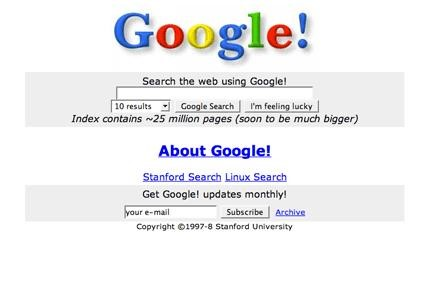
\includegraphics[width=0.97\linewidth]{2.3.1}
	\end{minipage}
	}
    \hfill
	\subfloat{
	\begin{minipage}[t]{0.5\linewidth}
	\centering
	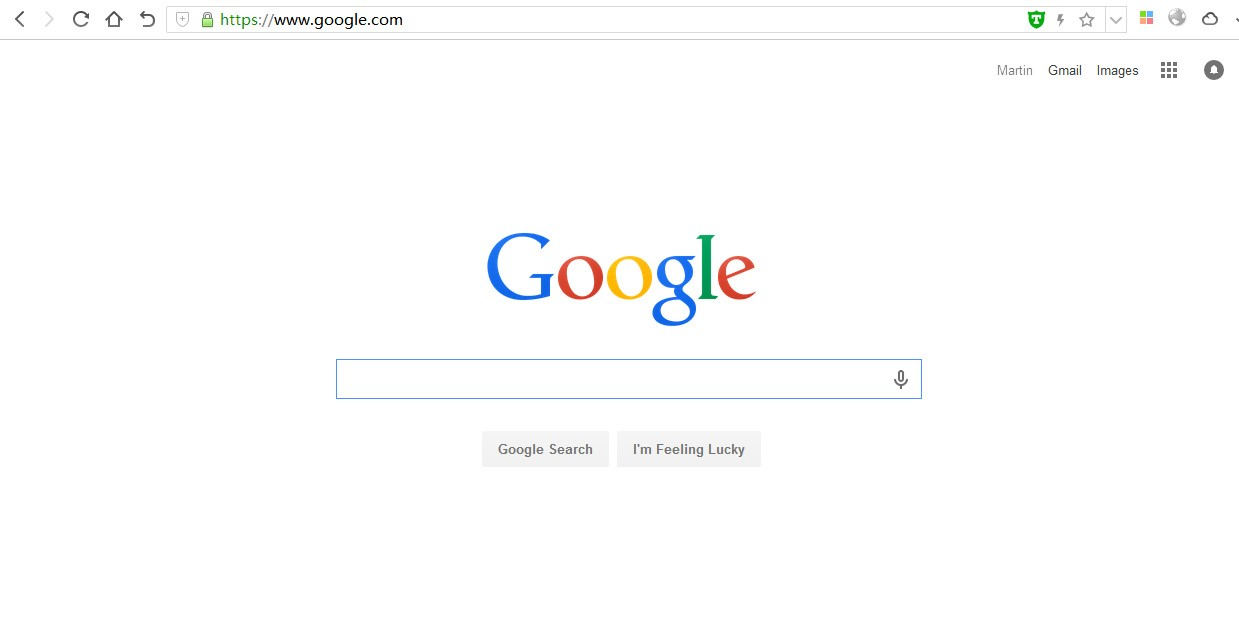
\includegraphics[width=0.97\linewidth]{2.3.2}
	\end{minipage}
	}
	\vspace{-1em}
\end{figure}
    \vspace{-0.8em}
    \begin{multicols}{2}
        \begin{enumerate}[label=\Alph*.]
            \item 第一个网站提供了对结果数量的控制
            \item 第二个网站只包含必要的UI组件
            \item 背景颜色
            \item 第二个网站的配色方案更优
        \end{enumerate}
    \end{multicols}
    \vspace{-1em}
\end{problem}

\begin{solution}
B.其他选项也都不同,但是最主要的区别还是下图去掉了很多多余的界面组件,使得“搜索框”这一系统入口变得更加明显。
\end{solution}


\begin{problem}
	提供加速器(如键盘快捷键等)的目的是为了提高系统的:
	\uline{D}    
    \vspace{-0.8em}
    \begin{multicols}{4}
        \begin{enumerate}[label=\Alph*.]
            \item 态度或喜爱程度
            \item 易学性
            \item 实用性
            \item 效率
        \end{enumerate}
    \end{multicols}
    \vspace{-1em}
\end{problem}

\begin{solution}
D.这一题比较简单,快捷键的主要特色是“快”。
\end{solution}


\begin{problem}
	能够帮助设计人员了解用户特定交互行为发生的原因的可用性工程方法是:
	\uline{A}    
    \vspace{-0.8em}
    \begin{multicols}{4}
        \begin{enumerate}[label=\Alph*.]
            \item 边做边说
            \item 用户和任务观察
            \item 启发式评估
            \item 场景
        \end{enumerate}
    \end{multicols}
    \vspace{-1em}
\end{problem}

\begin{solution}
A.边做边说是最有价值的单个可用性工程方法,简单的观察只能“知其然而不知其所以然”,通过让用户大声说出他们的想法,有助于明确用户遇到的具体问题。  B.该方法有助于了解用户的需要,通常用于早期需求获取阶段。  C.启发式评估的本质是专家模拟用户,性价比很高,但并不能替代对真实用户的观察和评估。  D.场景既可用于需求阶段,同人物角色一起描述需求;也可用于设计阶段,用于检验设计的细节。
\end{solution}
	\subsubsection*{\S 如何定义交互系统的需求和用户}
\setcounter{problemname}{0}

\begin{problem}
	‌以下哪一条是针对专家用户的设计原则:
    \vspace{-0.8em}
    \begin{multicols}{2}
        \begin{enumerate}[label=\Alph*.]
            \item 确保快速的响应时间
            \item 使用含义丰富的信息
            \item 减轻记忆负担
            \item 提供说明、对话框和在线帮助
        \end{enumerate}
    \end{multicols}
    \vspace{-1em}
\end{problem}



\begin{problem}
	以下关于短时记忆描述正确的是:  
    \vspace{-0.8em}
    \begin{multicols}{2}
        \begin{enumerate}[label=\Alph*.]
            \item 短时记忆的容量是有限的
            \item 短时记忆的容量很大,但容量有限
            \item 短时记忆的容量为零
            \item 短时记忆的容量是无限的
        \end{enumerate}
    \end{multicols}
    \vspace{-1em}
\end{problem}



\begin{problem}
	在进行界面设计时要注意对组件进行对齐,这是由于格式塔心理学中哪一条原则的影响:
    \vspace{-0.8em}
    \begin{multicols}{4}
        \begin{enumerate}[label=\Alph*.]
            \item 连续性
            \item 完整性
            \item 相似性
            \item 相近性
        \end{enumerate}
    \end{multicols}
    \vspace{-1em}
\end{problem}



\begin{problem}
	假设需要判断某应用程序的配色方案是否恰当。对于该测试任务,您将使用:  
    \vspace{-0.8em}
    \begin{multicols}{2}
        \begin{enumerate}[label=\Alph*.]
            \item 高保真模型
            \item 低保真模型
            \item 低保真和高保真模型均可
            \item 以上都错
        \end{enumerate}
    \end{multicols}
    \vspace{-1em}
\end{problem}



\begin{problem}
	以下关于“人物角色”描述正确的是:
    %\vspace{-0.8em}
    %\begin{multicols}{2}
        \begin{enumerate}[label=\Alph*.]
            \item 人物角色能够帮助克服当前数字产品开发中的很多问题
            \item 人物角色的概念以及使用都很简单
            \item 人物角色是设计人员编造的,并不是真实的人
            \item 人物角色不是特定于上下文的,所以它可以很容易地被重复使用
        \end{enumerate}
    %\end{multicols}
    %\vspace{-1em}
\end{problem}


	\subsubsection*{\S 如何开展交互设计}
\setcounter{problemname}{0}

\begin{problem}
	以下关于Allan Cooper提出的交互设计框架描述正确的是:
    %\vspace{-0.8em}
    %\begin{multicols}{2}
        \begin{enumerate}[label=\Alph*.]
            \item 验证性的场景剧本需要具备产品的很多细节信息
            \item 建议使用高保真草图序列的故事板来描述关键线路情景剧本
            \item 关键线路情景剧本必须在细节上严谨地描述每个主要交互的精确行为
            \item 交互设计框架可用于确定界面使用的颜色和风格
        \end{enumerate}
    %\end{multicols}
    %\vspace{-1em}
\end{problem}



\begin{problem}
	原型阶段跟在哪一个开发阶段的后面?
    \vspace{-0.8em}
    \begin{multicols}{4}
        \begin{enumerate}[label=\Alph*.]
            \item 评估
            \item 构建应用程序
            \item 理解用户需要
            \item 以上都不对
        \end{enumerate}
    \end{multicols}
    \vspace{-1em}
\end{problem}



\begin{problem}
	假设需要判断某应用程序的配色方案是否恰当。对于该测试任务,您将使用:
    \vspace{-0.8em}
    \begin{multicols}{2}
        \begin{enumerate}[label=\Alph*.]
            \item 高保真模型
            \item 低保真模型
            \item 低保真模型和高保真模型均可
            \item 低保真模型和高保真模型均不合适
        \end{enumerate}
    \end{multicols}
    \vspace{-1em}
\end{problem}



\begin{problem}
	‍对于主流用户很少使用,但自身需要更新的功能,可使用何种策略进行简化:
    \vspace{-0.8em}
    \begin{multicols}{4}
        \begin{enumerate}[label=\Alph*.]
            \item 转移
            \item 隐藏
            \item 删除
            \item 组织
        \end{enumerate}
    \end{multicols}
    \vspace{-1em}
\end{problem}



\begin{problem}
	‍关于交互设计模式,以下说法错误的是: 
    \vspace{-0.8em}
    \begin{multicols}{2}
        \begin{enumerate}[label=\Alph*.]
            \item 模式捕捉了良好设计中不变的特性
            \item 模式在交互设计中的应用还处于起步阶段
            \item 设计模式能帮助提供有价值、有用的设计思路
            \item 交互设计模式可以拿来即用,不需要修改
        \end{enumerate}
    \end{multicols}
    \vspace{-1em}
\end{problem}

	\subsubsection*{\S 如何对交互性能进行评价}
\setcounter{problemname}{0}

\begin{problem}
	‍以下关于交互评估描述错误的是:
	\uline{B}    
    \vspace{-0.8em}
    \begin{multicols}{2}
        \begin{enumerate}[label=\Alph*.]
            \item 评估过程需要严谨的设计
            \item 评估是设计过程中一个独立的阶段
            \item 评估不一定要遵循DECIDE框架
            \item 评估是系统化的数据搜集过程
        \end{enumerate}
    \end{multicols}
    \vspace{-1em}
\end{problem}

\begin{solution}
B.优秀的交互设计师应掌握如何在不同的开发阶段对系统的不同形式进行评估,因此不应将评估作为某个开发节点上的独立阶段。
\end{solution}


\begin{problem}
	‍为探索孩子们在一起是如何交谈的,并调查一种新型产品是否能帮助他们更积极地参与其中,可使用如下哪种技术:
	\uline{A}    
    \vspace{-0.8em}
    \begin{multicols}{4}
        \begin{enumerate}[label=\Alph*.]
            \item 实地研究
            \item 预测性评估
            \item 可用性测试
            \item DECIDE框架
        \end{enumerate}
    \end{multicols}
    \vspace{-1em}
\end{problem}

\begin{solution}
A.实地研究特别适合在真实环境中去理解用户的实际工作情形以及技术对他们的影响,特别适合于面向儿童和残疾人等特殊用户群体的理解和对产品开展评估工作。
\end{solution}


\begin{problem}
	‍关于启发式评估,以下论述正确的是:
	\uline{A}    
    %\vspace{-0.8em}
    %\begin{multicols}{4}
        \begin{enumerate}[label=\Alph*.]
            \item 启发式评估是一种基于专家的评估方法
            \item 启发式评估的结果只有界面中潜在的可用性问题列表
            \item 当界面元素存在多个可用性问题时,只需列举其中一个问题即可
            \item 专家应用启发式评估时,会从自身使用经验出发对界面进行判断
        \end{enumerate}
    %\end{multicols}
    %\vspace{-1em}
\end{problem}

\begin{solution}
B.启发式评估专家不仅能够罗列出产品中潜在的可用性问题,同时还能够针对问题给出建设性的修改意见和建议。  C.在开展启发式评估时应该尽可能罗列出所有存在的问题以及其违反的启发式原则。  D.在启发式评估中,专家应该使用基于角色扮演的方式去模拟目标用户使用产品的感受。
\end{solution}


\begin{problem}
	‍以下哪一条不属于用户测试前的准备步骤:
	\uline{D}    
    \vspace{-0.8em}
    \begin{multicols}{4}
        \begin{enumerate}[label=\Alph*.]
            \item 制定测试方案
            \item 选择参与用户
            \item 开展小规模测试
            \item 观察参与者
        \end{enumerate}
    \end{multicols}
    \vspace{-1em}
\end{problem}

\begin{solution}
D.用户测试的目的是对待测产品进行分析和评价,因而对实验人员的观察并不属于测试的相关工作。
\end{solution}


\begin{problem}
	‍‍以下论述正确的是:
	\uline{A}    
    %\vspace{-0.8em}
    %\begin{multicols}{4}
        \begin{enumerate}[label=\Alph*.]
            \item 原型既可以帮助发现设计问题,也可以用来帮助用户明确需求
            \item 评估不应该过早进行,因为此时系统还不够完善
            \item 高保真原型更接近系统,因而在评估中要尽可能使用高保真原型进行评估
            \item 纸质原型适用于产品开发过程中的任意阶段
        \end{enumerate}
    %\end{multicols}
    %\vspace{-1em}
\end{problem}

\begin{solution}
B.即便在还没有完成系统开发时,应用快速评估等方法去获取目标用户关于产品的意见和建议都是非常有益的。  C.高保真原型一方面由于制作较为困难,另一方面因其过于接近目标系统,从而会让用户误以为已经开发完成从而不再提出一些原则性的修改意见,同时开发人员也会误认为已找到了一个用户满意的设计,因而不再考虑其它方案。  D.通常在实际可运行的产品开发出来之后,就不建议继续使用纸质原型进行评价了。
\end{solution}
	\subsubsection*{\S 交互设计模型与理论}
\setcounter{problemname}{0}

\begin{problem}
	‍‌以下关于任务分析描述错误的是:
	\uline{C}    
    %\vspace{-0.8em}
    %\begin{multicols}{4}
        \begin{enumerate}[label=\Alph*.]
            \item 层次化任务分析采用的是“分而治之”的方法
            \item 任务分析对于改善用户体验至关重要
            \item 只要肯花时间,总是可以实现完善的任务分析
            \item 层次化任务分析是人因工效学领域中最广泛使用的方法
        \end{enumerate}
    %\end{multicols}
    %\vspace{-1em}
\end{problem}

\begin{solution}
C.任务分析没有统一的标准答案,因而也很难定义什么样的任务分析是完善的。
\end{solution}


\begin{problem}
	GOMS的全称是什么?
	\uline{A}    
    \vspace{-0.8em}
    \begin{multicols}{2}
        \begin{enumerate}[label=\Alph*.]
            \item Goals, operation, methods and selection rules
            \item Goals, objects, models and selection rules
            \item Goals, operations, methods and state rules
            \item Goals, operations, models and state rules
        \end{enumerate}
    \end{multicols}
    \vspace{-1em}
\end{problem}

\begin{solution}
A.目标、操作、方法和选择规则。
\end{solution}


\begin{problem}
	以下关于击键层次模型描述不正确的是:
	\uline{B}    
    %\vspace{-0.8em}
    %\begin{multicols}{2}
        \begin{enumerate}[label=\Alph*.]
            \item 击键层次模型预测假设交互过程中没有错误发生
            \item 使用击键层次模型预测的难点在于对操作路径的分析
            \item 击键层次模型用于预测指点任务的完成时间
            \item 击键层次模型预测的是无干扰情况下完成任务的时间
        \end{enumerate}
    %\end{multicols}
    %\vspace{-1em}
\end{problem}

\begin{solution}
B.使用击键层次模型的难点在于M操作符的使用,即在哪些操作之前需要引入一个思维过程。
\end{solution}


\begin{problem}
	以下关于Fitts定律描述不正确的是:
	\uline{C}    
    %\vspace{-0.8em}
    %\begin{multicols}{2}
        \begin{enumerate}[label=\Alph*.]
            \item Fitts定律对于图形用户界面应用开发具有重要指导意义
            \item Fitts定律也可用于指导现实生活中的产品设计
            \item Fitts定律可以预测任意交互操作的完成时间
            \item Fitts定律是一种预测模型
        \end{enumerate}
    %\end{multicols}
    %\vspace{-1em}
\end{problem}

\begin{solution}
C. Fitts定律只能够预测指点型任务的完成时间,即应用某种操作设备(鼠标、触摸板、手指等)访问屏幕某个区域或对象的时间。
\end{solution}


\begin{problem}
	以下关于预测模型描述正确的是:
	\uline{A}    
    %\vspace{-0.8em}
    %\begin{multicols}{2}
        \begin{enumerate}[label=\Alph*.]
            \item 预测模型可用于比较不同的应用软件和设备
            \item 预测模型只能预测任务的完成时间
            \item 预测模型预测的任务完成时间和实际用户的任务执行时间一致
            \item 预测模型能够对所有任务的完成情况进行预测
        \end{enumerate}
    %\end{multicols}
    %\vspace{-1em}
\end{problem}

\begin{solution}
B.预测模型不仅能够预测任务的完成时间,还能对任务的完成策略(如次序)进行预测。  C.预测模型预测的是专家用户在没有任何错误的情况下完成任务的时间,通常与真实用户的实际任务执行时间存在出入。  D.预测模型只能预测“认知-动作型”任务的完成情况。
\end{solution}

\end{document}

% \begin{compactenum}
%     \item 
% \end{compactenum}


% \begin{figure}[H]
%     \vspace{-0.5em}
% 	\centering
% 	\includegraphics[width=0.4\textwidth]{images/}
% 	\caption{}
%     \label{}
%     \vspace{-1em}
% \end{figure}


% \vspace{-0.8em}
% \begin{multicols}{2}
%     \begin{itemize}
%         \item 
%     \end{itemize}
% \end{multicols}
% \vspace{-1em}


% \vspace{-0.5em}
% \begin{spacing}{1.2}
%     \centering
%     \begin{longtable}{|W{c}{2.5cm}|W{c}{3.8cm}|W{c}{4.2cm}|m{4cm}<{\centering}|}
% 		表格内容
% 		表头居中方式  \multicolumn{1}{c|}{表头内容} 
%     \end{longtable}
% 	\end{spacing}
% \vspace{-1em}


% \begin{figure}[htbp]
% 	\setcounter{subfigure}{0}
% 	\centering
% 	\vspace{-0.5em}	
% 	\subfloat[]{
% 	\begin{minipage}[t]{0.33\linewidth}
% 	\centering
% 	\includegraphics[width=0.97\linewidth]{}
% 	\caption{}
%     \label{}
% 	\end{minipage}
% 	}
% 	\subfloat[]{
% 	\begin{minipage}[t]{0.33\linewidth}
% 	\centering
% 	\includegraphics[width=0.97\linewidth]{}
% 	\caption{}
%     \label{}
% 	\end{minipage}
% 	}
% 	\centering
% 	\vspace{-1em}
% 	\caption{}
% \end{figure}


% \begin{wraptable}{r}{6.5cm}
%     \centering
%     \vspace{-1.5em}
%     \begin{tabular}{|c|c|}
%     \hline
%     期望的确定性 & 确定性因子 \\ \hline
%     95\% & 1.960  \\ \hline
%     90\% & 1.645  \\ \hline
%     85\% & 1.281  \\ \hline
%     \end{tabular}
%     \caption*{常见的确定性因子}
%     \vspace{-1.5em}
% \end{wraptable}


% \vspace{-0.5em}
% \begin{shaded}

% \end{shaded}
% \vspace{-1em}
